
% Copyright (c) 2015 - 2019 Mario Mlačak, mmlacak@gmail.com
% Licensed and published as Public Domain work.

% Miranda's veil chapter ==============================================
\chapter*{Miranda's veil}
\addcontentsline{toc}{chapter}{Miranda's veil}

\begin{flushright}
\parbox{0.8\textwidth}{
\emph{Under all that we think, lives all we believe, like the ultimate veil of our spirits. \\
\hspace*{\fill}{\textperiodcentered \textperiodcentered \textperiodcentered \hspace*{0.2em} Antonio Machado} } }
\end{flushright}

\noindent
Miranda's veil is chess variant which is played on 16 x 16 board, with
white and dark violet fields and light magenta and indigo pieces. In
algebraic notation, columns are enumerated from 'a' to 'p', and rows
are enumerated from '1' to '16'. A new piece is introduced, Wave.

\clearpage % ..........................................................
% Wave ****************************************************************

\section*{Wave}
\addcontentsline{toc}{section}{Wave}

% \vspace*{-2.0ex} % Wonders of LaTeX formatting.
\noindent
\begin{wrapfigure}[12]{l}{0.4\textwidth}
\centering
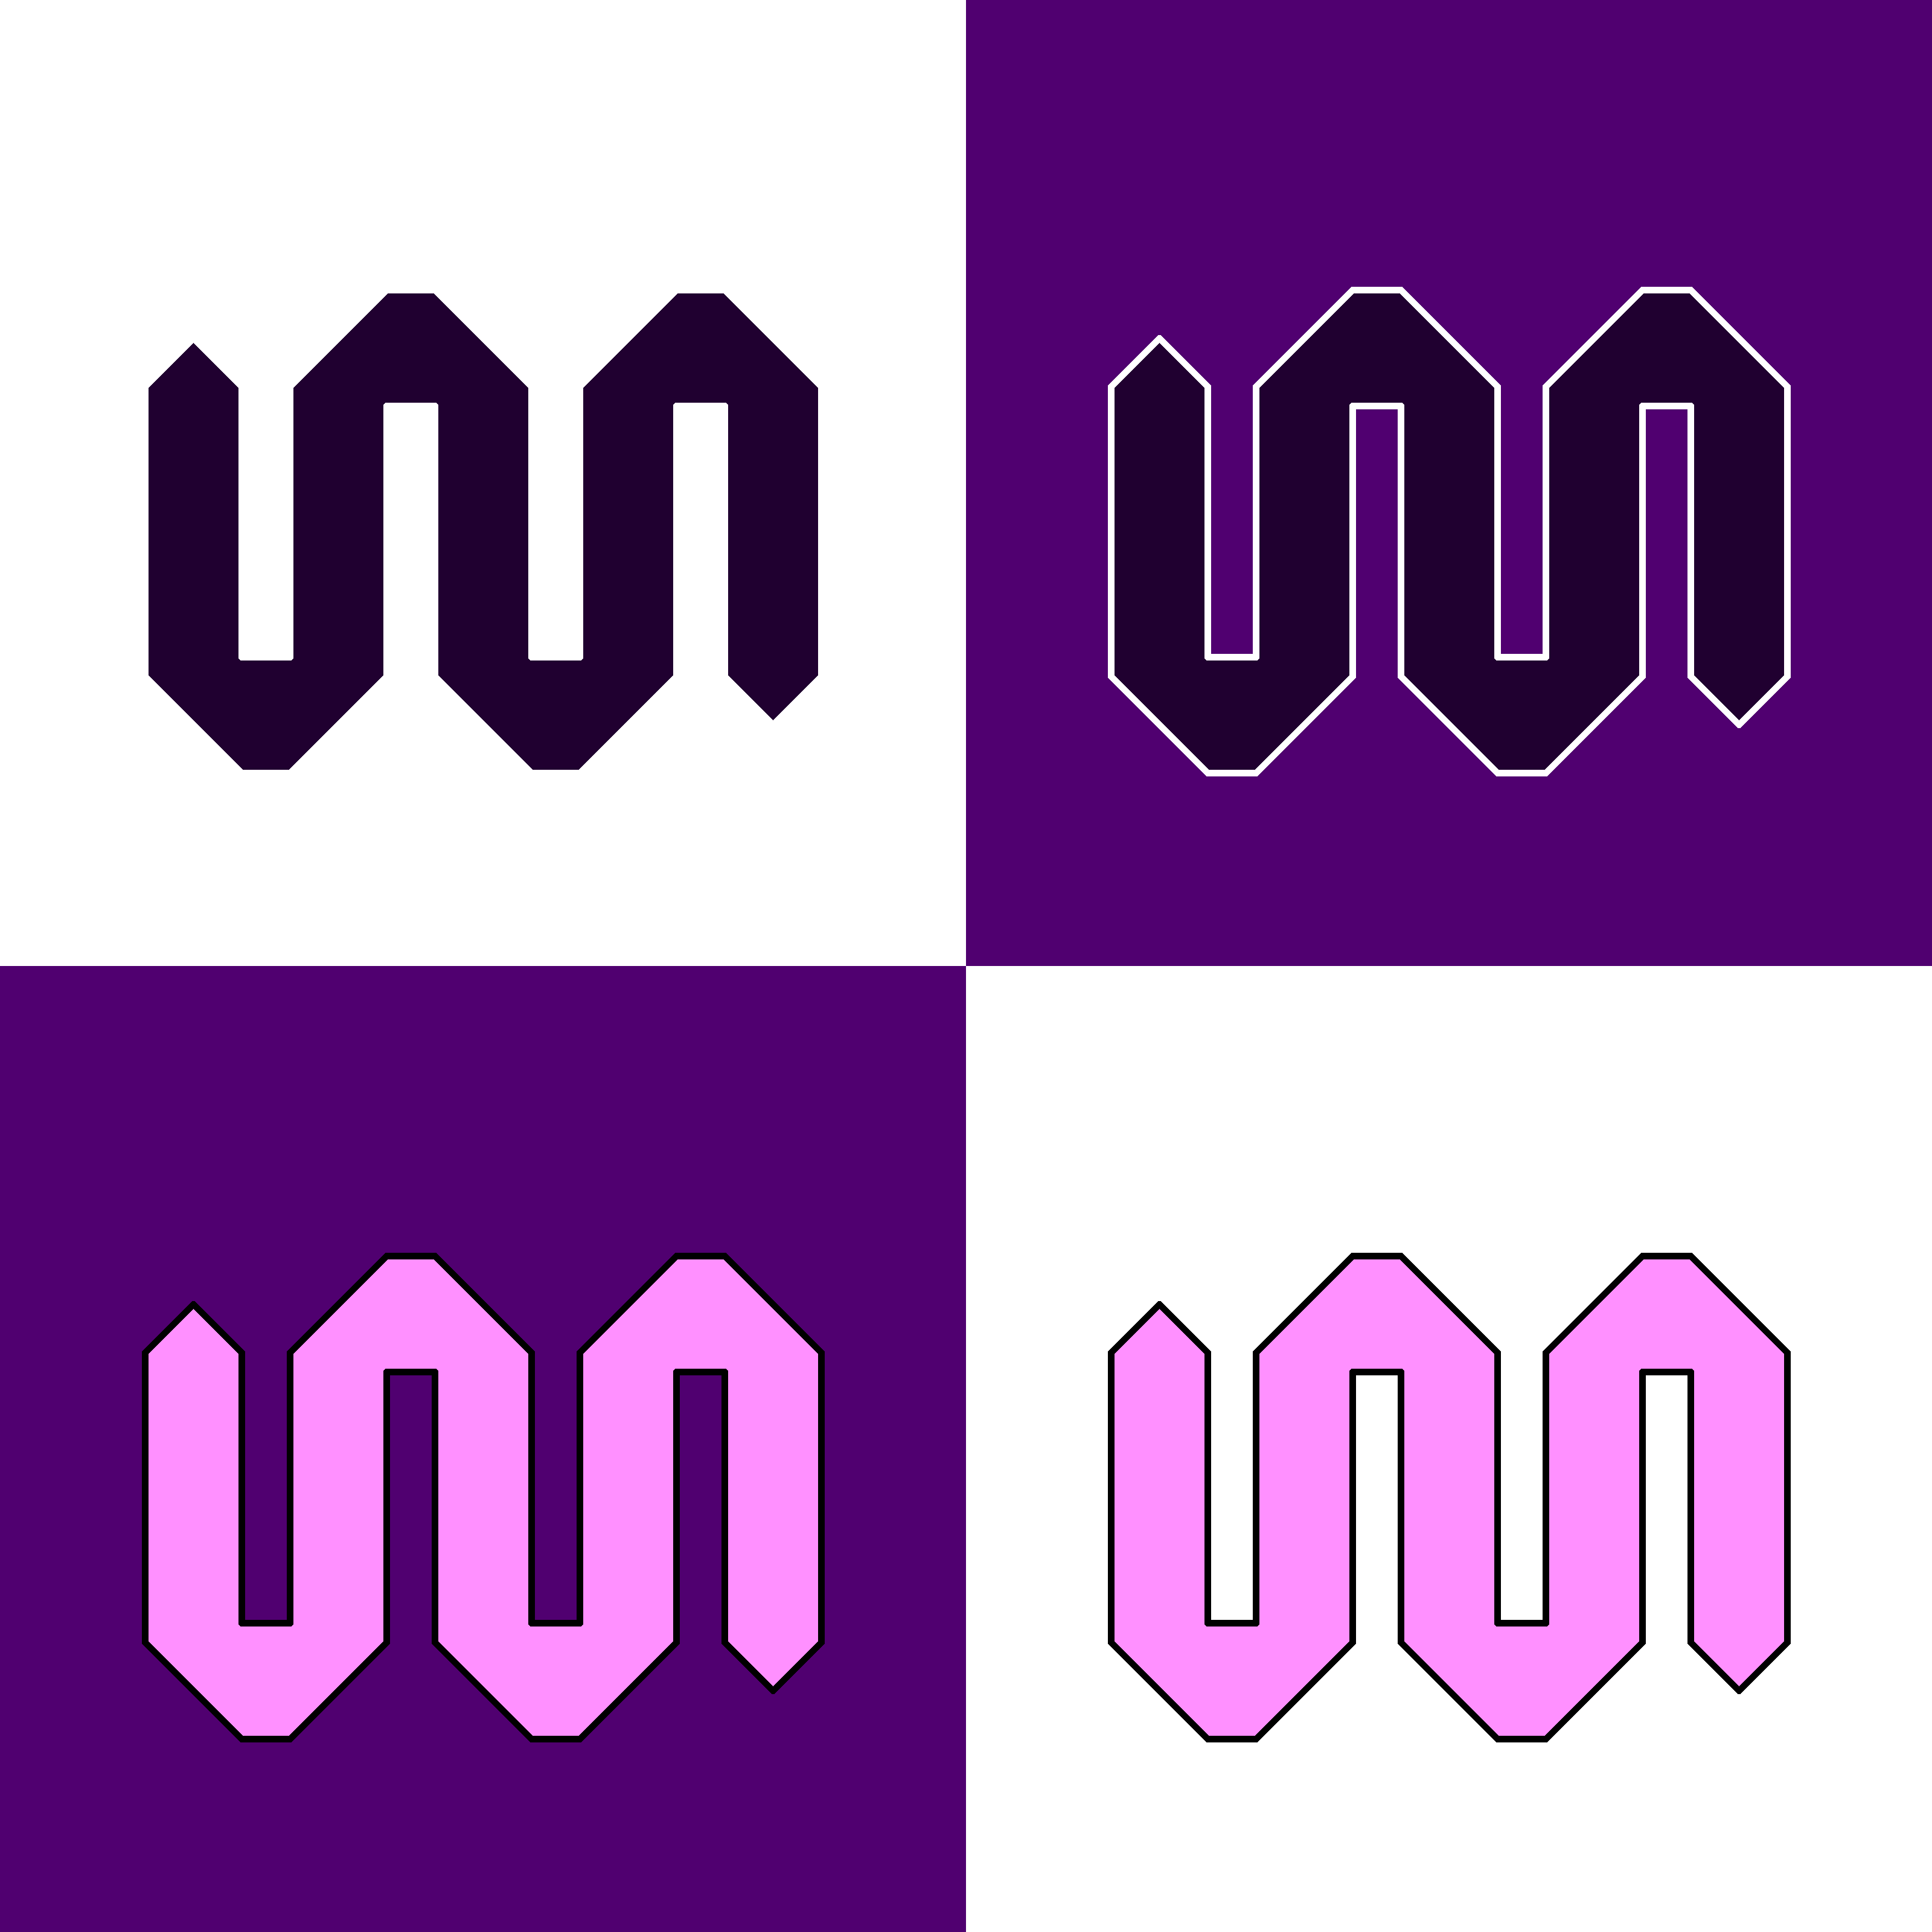
\includegraphics[width=0.4\textwidth, keepaspectratio=true]{pieces/10_wave.png}
\caption{Wave}
\label{fig:10_wave}
\end{wrapfigure}
Wave is passive piece, it has to be activated before it can move. Activation
is done in the same way as with Pyramid. Own piece has to capture field at
which Wave is located before Wave can move.

Wave can be activated even if activating piece has no momentum. Wave does not
use received momentum for moving, and isn't limited by it.
Wave can move freely even if it has no momentum. Wave is not blocked by any piece,
it can continue its' movement freely as if there are no pieces on board at all.

After activation Wave moves like activating piece, over piece's step- or capture-
fields, depending where it was activated. Wave can make multiple steps, in the
same way activating piece does, even if activating piece can make only one. Note,
Wave can choose direction on the first step, which cannot be changed later. For
details see \hyperref[sec:Definitions/Movement of Wave]{'Movement of Wave'}.

Wave cannot capture any piece. Thus, Wave cannot check nor checkmate opponent's
King.

Wave can activate any own piece, except King, if it has momentum. Wave can
also activate other Wave, own or opponent's, even if it has no momentum. In
all cases, Wave transfers all received momentum to activated piece.

In algebraic notation symbol for Wave is 'W'.

\clearpage % ..........................................................
% Activation ----------------------------------------------------------

\subsection*{Activation}
\addcontentsline{toc}{subsection}{Activation}

\vspace*{-2.0ex}
\noindent
% \begin{figure}[t]
\begin{figure}[h]
\includegraphics[width=1.0\textwidth, keepaspectratio=true]{examples/10_mv/scn_mv_01_move_wave_init.png}
\caption{Wave activation}
\label{fig:scn_mv_01_move_wave_init}
% \centering
\end{figure}

Above, after activation Wave could move the same way Knight does, over multiple
step-fields. Once Wave starts moving in a chosen direction, it cannot be changed.
So, in this case Wave would move as Pegasus does. Wave does not spend received
momentum while moving, and would transfer it entirely to any piece it activates.

\clearpage % ..........................................................

\noindent
% \begin{figure}[t]
\begin{figure}[h]
\includegraphics[width=1.0\textwidth, keepaspectratio=true]{examples/10_mv/scn_mv_02_move_wave_activated.png}
\caption{Wave activated}
\label{fig:scn_mv_02_move_wave_activated}
% \centering
\end{figure}

Wave can move unhindered by any piece, even on step-fields (green arrows). Wave
can also activate pieces (blue arrows) obscured by others, for instance light
Pyramid which is out of reach for regular Pegasus. Wave cannot activate Kings nor
opponent's pieces (red arrows), except dark Wave. \\
Again, Wave cannot change direction of movement after first step. For instance,
upon reaching step-field 5, it cannot change direction to 5c, or any other
greyed-out arrow.

\clearpage % ..........................................................

\noindent
% \begin{figure}[t]
\begin{figure}[h]
\includegraphics[width=1.0\textwidth, keepaspectratio=true]{examples/10_mv/scn_mv_03_move_wave_finished.png}
\caption{Wave finished}
\label{fig:scn_mv_03_move_wave_finished}
% \centering
\end{figure}

Greyed-out arrows show steps Wave have taken in its' ply. Activated Bishop
now continues the move according to own rules of movement, i.e. diagonally.
Note that it's restricted by momentum received, and thus can make only one
step, i.e. can move for only one field.

% ---------------------------------------------------------- Activation
\clearpage % ..........................................................
% Cascading Waves -----------------------------------------------------

\subsection*{Cascading Waves}
\addcontentsline{toc}{subsection}{Cascading Waves}

\noindent
\begin{wrapfigure}[13]{l}{0.5625\textwidth}
\centering
\includegraphics[width=0.5625\textwidth, keepaspectratio=true]{examples/10_mv/scn_mv_04_cascading_rook.png}
\caption{Rook starting cascade}
\label{fig:scn_mv_04_cascading_rook}
\end{wrapfigure}
Cascading Waves refers to a move in which two or more Waves have been displaced.
For example, Wave can activate another Wave. Wave can also activate active
piece (or Pyramid), which can then activate another Wave.

On the left, Rook is about to activate Wave 1, giving it momentum of 4.

\vspace*{0.05\textheight}
\noindent
\begin{wrapfigure}[12]{r}{0.5625\textwidth}
\centering
\includegraphics[width=0.5625\textwidth, keepaspectratio=true]{examples/10_mv/scn_mv_05_cascading_wave_1.png}
\caption{Wave 1 cascading}
\label{fig:scn_mv_05_cascading_wave_1}
\end{wrapfigure}
Activated Wave 1 inherits rules of movement from activating piece, and so now
moves as Rook would. It's not obstructed with any piece in its' way, nor it's
limited by received momentum, i.e. it can move further than just 4 fields away.
Wave 1 can also activate Wave 2.

\clearpage % ..........................................................

\noindent
\begin{wrapfigure}[13]{l}{0.5625\textwidth}
\centering
\includegraphics[width=0.5625\textwidth, keepaspectratio=true]{examples/10_mv/scn_mv_06_cascading_wave_2.png}
\caption{Wave 2 cascading}
\label{fig:scn_mv_06_cascading_wave_2}
\end{wrapfigure}
Activated Wave 2 inherits rules of movement from activating piece (in this
case Wave 1), and so too moves as Rook would. Wave 2 also received momentum
of 4. Again, it's not obstructed by any piece, nor it's limited by received
momentum. Wave 2 can also activate either Queen or Rook.

\vspace*{0.075\textheight}
\noindent
\begin{wrapfigure}[9]{r}{0.5625\textwidth}
\centering
\includegraphics[width=0.5625\textwidth, keepaspectratio=true]{examples/10_mv/scn_mv_07_cascading_rook_2nd_time.png}
\caption{Rook, 2nd cascading}
\label{fig:scn_mv_07_cascading_rook_2nd_time}
\end{wrapfigure}
Rook is now activated, but it is limited by momentum received, i.e. it can
move at most 4 fields away. Naturaly, Rook is obstructed by surrounding pieces,
i.e. it can't move past Wave 1. Rook can activate Wave 1.

\clearpage % ..........................................................

\noindent
\begin{wrapfigure}[10]{l}{0.5625\textwidth}
\centering
\includegraphics[width=0.5625\textwidth, keepaspectratio=true]{examples/10_mv/scn_mv_08_cascading_wave_1_2nd_time.png}
\caption{Wave 1, 2nd cascading}
\label{fig:scn_mv_08_cascading_wave_1_2nd_time}
\end{wrapfigure}
Activated Wave 1 received momentum of 2 and rules of movement from Rook. Again,
Wave 1 is not obstructed by any piece, nor it is limited by received momentum.
Wave 1 can also activate either Queen or Wave 2.

\vspace*{0.155\textheight}
\noindent
\begin{wrapfigure}[10]{r}{0.5625\textwidth}
\centering
\includegraphics[width=0.5625\textwidth, keepaspectratio=true]{examples/10_mv/scn_mv_09_cascading_queen.png}
\caption{Queen cascading}
\label{fig:scn_mv_09_cascading_queen}
\end{wrapfigure}
Activated Queen received momentum of 2, it can move at most 2 fields away.
Queen can also activate Wave 2, giving it momentum of 0.

\clearpage % ..........................................................

\noindent
\begin{wrapfigure}[7]{l}{0.5625\textwidth}
\centering
\includegraphics[width=0.5625\textwidth, keepaspectratio=true]{examples/10_mv/scn_mv_10_cascading_wave_2_2nd_time.png}
\caption{Wave 2, 2nd cascading}
\label{fig:scn_mv_10_cascading_wave_2_2nd_time}
\end{wrapfigure}
Activated Wave 2 received rules of movement from Queen, and 0 momentum.
Note, since Wave 2 has no momentum it can't activate Rook, only Wave 1.

\vspace*{0.245\textheight}
\noindent
\begin{wrapfigure}[9]{r}{0.5625\textwidth}
\centering
\includegraphics[width=0.5625\textwidth, keepaspectratio=true]{examples/10_mv/scn_mv_11_cascading_wave_1_3rd_time.png}
\caption{Wave 1, 3rd cascading}
\label{fig:scn_mv_11_cascading_wave_1_3rd_time}
\end{wrapfigure}
Activated Wave 1 inherits rules of movement from activating piece (Wave 2),
meaning Wave 1 too now moves as Queen would. Due to no momentum, Wave 1 can't
activate neither Queen nor Rook.

\clearpage % ..........................................................

\noindent
\begin{wrapfigure}[3]{l}{0.5625\textwidth}
\centering
\includegraphics[width=0.5625\textwidth, keepaspectratio=true]{examples/10_mv/scn_mv_12_cascading_end.png}
\caption{Wave 1, end cascading}
\label{fig:scn_mv_12_cascading_end}
\end{wrapfigure}
Wave 1 end this rather long cascade by settling past Rook.

\vspace*{0.345\textheight}
In a cascade, Wave is not limited by received momentum, nor it's obstructed by
other pieces on board.

Wave inherts rules of movement from activating piece, but can make multiple
steps, even if activating piece can make only one. All other pieces moves
according to their own rules, and are restricted by momentum received. For
details see \hyperref[sec:Definitions/Movement of Wave]{'Movement of Wave'} in
Definitions.

During cascade, after each ply (movement of a piece) activation takes place
according to current positions of pieces on the board, just as it would at the
beginning of the move.

\label{txt:Miranda's veil/Cascading Waves/Push-pull activation}
This makes it possible, in the same cascade, to activate piece which started it
(Rook in this example). Such cascade is said to feature push-pull activation.
It's also possible to reactivate other (non-initiating) pieces in the same
cascade. Here, Wave 1 was reactivated 3 times, while Wave 2 was reactivated
twice.

% ----------------------------------------------------- Cascading Waves
\clearpage % ..........................................................
% Cascading opponent --------------------------------------------------

\subsection*{Cascading opponent}
\addcontentsline{toc}{subsection}{Cascading opponent}

\noindent
\begin{wrapfigure}[10]{l}{0.5625\textwidth}
\centering
\includegraphics[width=0.5625\textwidth, keepaspectratio=true]{examples/10_mv/scn_mv_13_casc_oppo_light_queen.png}
\caption{Light Queen starting cascade}
\label{fig:scn_mv_13_casc_oppo_light_queen}
\end{wrapfigure}
Cascading opponent refers to a move in which opponent's Wave has been displaced,
potentially other opponent's pieces.

On the left, light Queen is about to activate light Wave, giving it momentum of 3.

\vspace*{0.155\textheight}
\noindent
\begin{wrapfigure}[5]{r}{0.5625\textwidth}
\centering
\includegraphics[width=0.5625\textwidth, keepaspectratio=true]{examples/10_mv/scn_mv_14_casc_oppo_light_wave.png}
\caption{Light Wave}
\label{fig:scn_mv_14_casc_oppo_light_wave}
\end{wrapfigure}
Activated light Wave can activate dark Wave, but can't interact with dark Queen in
any way.

\clearpage % ..........................................................

\noindent
\begin{wrapfigure}[5]{l}{0.5625\textwidth}
\centering
\includegraphics[width=0.5625\textwidth, keepaspectratio=true]{examples/10_mv/scn_mv_15_casc_oppo_dark_wave.png}
\caption{Dark Wave}
\label{fig:scn_mv_15_casc_oppo_dark_wave}
\end{wrapfigure}
Activated dark Wave now can activate dark Queen, but cannot interact with light Queen
in any way.

\vspace*{0.315\textheight}
\noindent
\begin{wrapfigure}[13]{r}{0.5625\textwidth}
\centering
\includegraphics[width=0.5625\textwidth, keepaspectratio=true]{examples/10_mv/scn_mv_16_casc_oppo_dark_queen.png}
\caption{Dark Queen}
\label{fig:scn_mv_16_casc_oppo_dark_queen}
\end{wrapfigure}
Activated dark Queen is limited to momentum transferred to it, i.e. 3. Dark Queen
cannot activate light Wave. Just as it could in ordinary, non-cascading move dark
Queen can capture either light Wave or light Queen. Also, dark Queen is obstructed
by pieces present on board.

\clearpage % ..........................................................

\noindent
\begin{wrapfigure}[4]{l}{0.5625\textwidth}
\centering
\includegraphics[width=0.5625\textwidth, keepaspectratio=true]{examples/10_mv/scn_mv_17_casc_oppo_end.png}
\caption{Cascading opponent end}
\label{fig:scn_mv_17_casc_oppo_end}
\end{wrapfigure}
This example of cascading opponent ends with dark Queen capturing light Queen.

\vspace*{0.355\textheight}
In summary, during cascade opponent's pieces retain all of their normal behavior,
most notably capturing their opponent's (in cascade, that means your own!) pieces.

This behavior retention include checking and checkmating their opponent's (again,
your own) King, en passant, promotion of their own pieces (if their Pyramid has
been activated), etc. This list includes all other movements, features described
later in this book.

Plies which cannot be performed by opponent's pieces during cascade are those
involving opponent's King, including castling, as that would require activation
of opponent's King, which is not allowed.

% -------------------------------------------------- Cascading opponent
\clearpage % ..........................................................
% Activating Pawn -----------------------------------------------------

\subsection*{Activating Pawn}
\addcontentsline{toc}{subsection}{Activating Pawn}

\noindent
\begin{figure}[!h]
% \begin{figure}[!t]
\includegraphics[width=1.0\textwidth, keepaspectratio=true]{examples/10_mv/scn_mv_18_activating_rush_pawn_init.png}
\caption{Activating Pawns}
\label{fig:scn_mv_18_activating_rush_pawn_init}
% \centering
\end{figure}

Activating Pawn in its' initial position gives it ability to capture opponent's
piece, or rush, i.e. perform longer initial movement. Pawn can be rushed only for
momentum received, but no more than longest rush move available, in this variant
up to (and including) 6 fields.

\clearpage % ..........................................................

\noindent
\begin{figure}[!h]
% \begin{figure}[!t]
\includegraphics[width=1.0\textwidth, keepaspectratio=true]{examples/10_mv/scn_mv_19_activating_rush_pawn_end.png}
\caption{Pawns activated}
\label{fig:scn_mv_19_activating_rush_pawn_end}
% \centering
\end{figure}

Pawn 1 received 4 momentum, and so when rushing it the furthest 2 fields are out
of reach. Pawn 2 had 13 momentum, but could use only 6 for rush, since this is the
longest rush movement available in this variant.

% ----------------------------------------------------- Activating Pawn
\clearpage % ..........................................................

\subsection*{Activation by Pawn}
\addcontentsline{toc}{subsection}{Activation by Pawn}

\vspace*{-1.0ex} % Does space after title depends on size of paragraph that follows?
\noindent
\begin{figure}[!h]
% \begin{figure}[!t]
\includegraphics[width=1.0\textwidth, keepaspectratio=true]{examples/10_mv/scn_mv_20_wave_activation_by_step_pawn.png}
\caption{Pawn activates Wave on step-field}
\label{fig:scn_mv_20_wave_activation_by_step_pawn}
% \centering
\end{figure}

Pawn can activate Wave on its' step-fields. Ordinary step would give 1 momentum to
Wave (Pawn 1), while rushed Pawn would give count of travelled-over step-fields as
momentum, in this case 3 (Pawn 2). Note, rushed Pawn has to capture field at which
Wave is located, and is blocked from rushing any further.

\clearpage % ..........................................................

\noindent
\begin{figure}[!h]
% \begin{figure}[!t]
\includegraphics[width=1.0\textwidth, keepaspectratio=true]{examples/10_mv/scn_mv_21_wave_activated_by_step_pawn.png}
\caption{Wave activated on Pawn's step-field}
\label{fig:scn_mv_21_wave_activated_by_step_pawn}
% \centering
\end{figure}

In all cases, Wave activated on Pawn's step-fields can move only forward, until the end
of the board. Either Wave could also activate light Knight or light Bishop, transferring
to them received momentum (1 and 3, respectively). Wave cannot change its' direction to
Pawn's capture-fields, even if pieces are present on them. So, Wave cannot activate neither
opponent's piece (dark Wave), nor own (Pawn 3).

\clearpage % ..........................................................

\noindent
\begin{figure}[!h]
% \begin{figure}[!t]
\includegraphics[width=1.0\textwidth, keepaspectratio=true]{examples/10_mv/scn_mv_22_wave_activation_by_capture_pawn.png}
\caption{Pawn activates Wave on capture-field}
\label{fig:scn_mv_22_wave_activation_by_capture_pawn}
% \centering
\end{figure}

Wave can be activated by Pawn on its' capture-field, receiving 1 momentum.

\clearpage % ..........................................................

\noindent
\begin{figure}[!h]
% \begin{figure}[!t]
\includegraphics[width=1.0\textwidth, keepaspectratio=true]{examples/10_mv/scn_mv_23_wave_activated_by_capture_pawn.png}
\caption{Wave activated on Pawn's capture-field}
\label{fig:scn_mv_23_wave_activated_by_capture_pawn}
% \centering
\end{figure}

Activated Wave can move forward diagonally, either to the left or to the right, until the
end of the board, regardless if capture-fields are empty, or if own or opponent's pieces are
present. Wave could also activate either light Bishop or light Knight, giving it received 1
momentum. Wave cannot change direction to Pawn's step-fields, and so can't activate light
Pegasus.

\clearpage % ..........................................................

\subsection*{Activation by Unicorn}
\addcontentsline{toc}{subsection}{Activation by Unicorn}

\noindent
\begin{figure}[!h]
% \begin{figure}[!t]
\includegraphics[width=1.0\textwidth, keepaspectratio=true]{examples/10_mv/scn_mv_24_wave_activation_by_unicorn.png}
\caption{Unicorn activates Wave}
\label{fig:scn_mv_24_wave_activation_by_unicorn}
% \centering
\end{figure}

... Unicorn ...

\clearpage % ..........................................................

\noindent
\begin{figure}[!h]
% \begin{figure}[!t]
\includegraphics[width=1.0\textwidth, keepaspectratio=true]{examples/10_mv/scn_mv_25_wave_activated_by_unicorn.png}
\caption{Wave activated by Unicorn}
\label{fig:scn_mv_25_wave_activated_by_unicorn}
% \centering
\end{figure}

... Unicorn ...

\clearpage % ..........................................................

\subsection*{Out of board steps}
\addcontentsline{toc}{subsection}{Out of board steps}

\vspace*{-1.0ex} % Does space after title depends on size of paragraph that follows?
\noindent
\begin{figure}[!h]
% \begin{figure}[!t]
\includegraphics[width=1.0\textwidth, keepaspectratio=true]{examples/10_mv/scn_mv_26_wave_off_board.png}
\caption{Wave off-board steps}
\label{fig:scn_mv_26_wave_off_board}
% \centering
\end{figure}

Here, light grey fields are virtual fields extending existing chessboard.
For Wave, it's legal to step outside of a board, and all subsequent steps
are also legal, as long as its' ply ends on a board. So, Wave activated by
Unicorn can reach fields 1 and 2, even though it stepped outside of the
board. It is illegal for any piece to end its' ply outside of a board.

% **************************************************************** Wave
\clearpage % ..........................................................

\section*{Promotion}
\addcontentsline{toc}{section}{Promotion}

Promotion is non enforced, delayed variety, i.e. it's the same as in
\hyperref[sec:Age of Aquarius/Promotion]{previous chess variant}, Age of Aquarius.

\clearpage % ..........................................................

\section*{En passant}
\addcontentsline{toc}{section}{En passant}

\noindent
\begin{wrapfigure}{l}{0.4\textwidth}
\centering
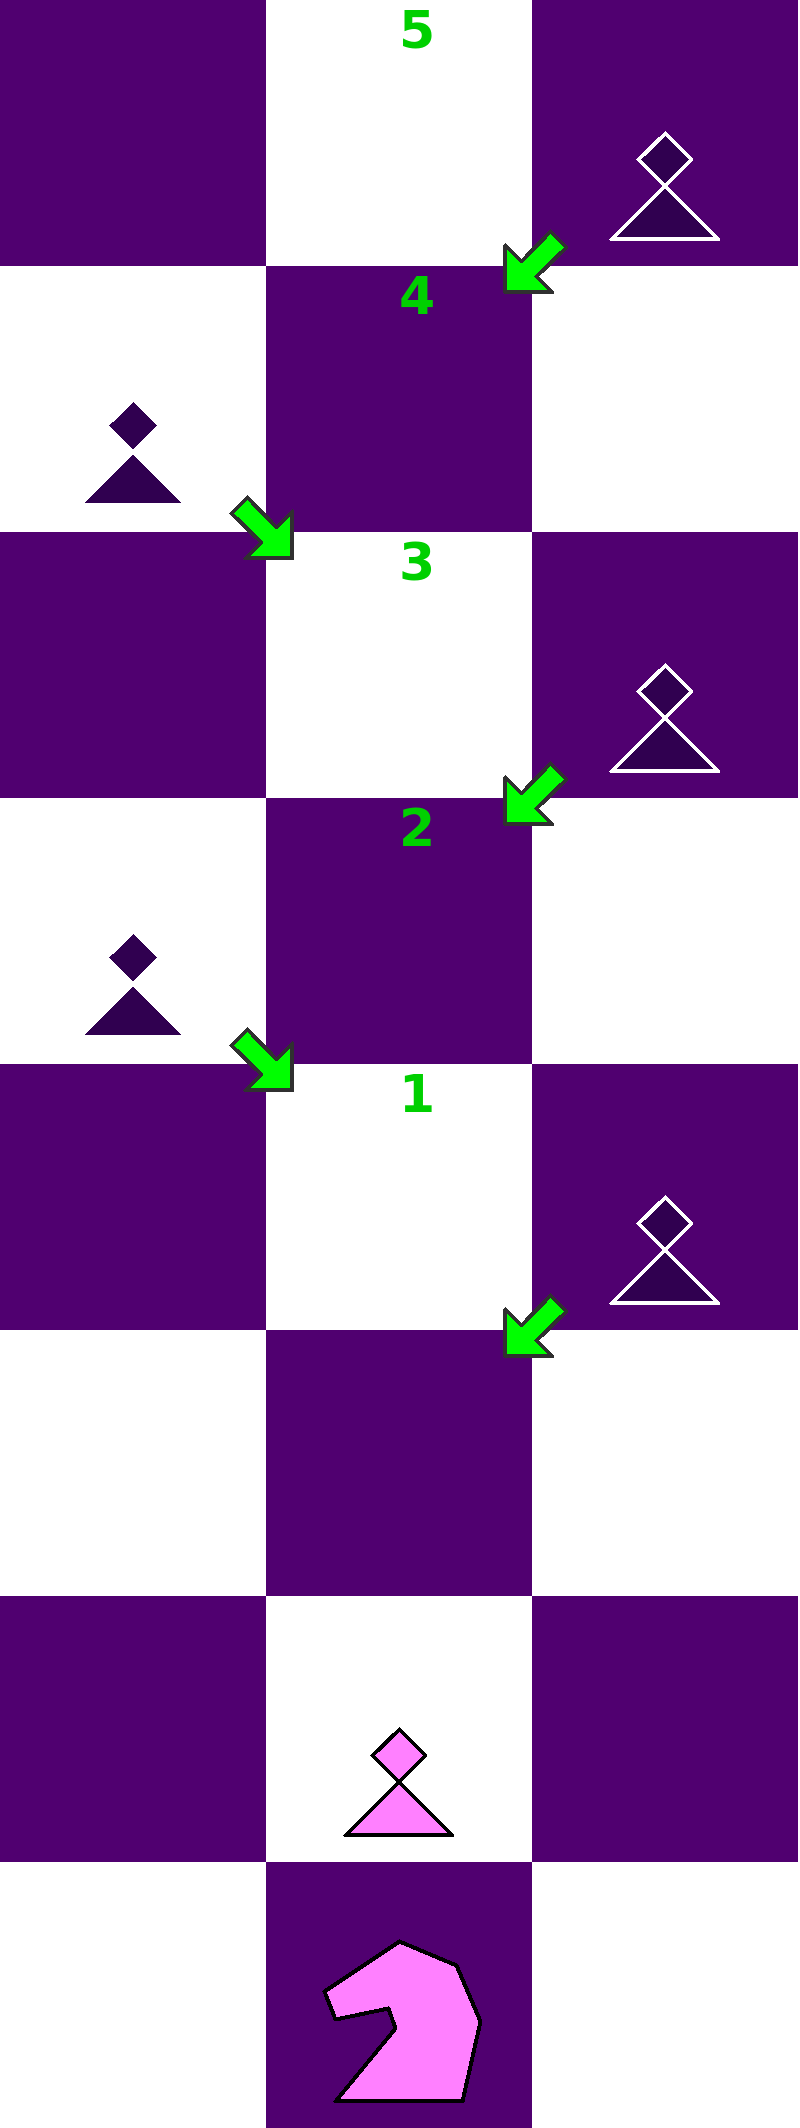
\includegraphics[width=0.1875\textwidth, keepaspectratio=true]{en_passants/10_miranda_s_veil_en_passant.png}
\caption{En passant}
\label{fig:10_miranda_s_veil_en_passant}
\end{wrapfigure}
Rush and en passant are identical to those in Classic Chess, only difference
is that Pawn can now move longer on initial turn, up to 6 fields in this
variant.

\clearpage % ..........................................................

\section*{Castling}
\addcontentsline{toc}{section}{Castling}

Castling is the same as in Classical Chess, only difference is that King can move between 2 and 6 fields across.
All other constraints from Classical Chess still applies.

\noindent
\begin{figure}[!h]
% \begin{figure}[!t]
\includegraphics[width=1.0\textwidth, keepaspectratio=true]{castlings/10_mv/miranda_s_veil_castling.png}
\caption{Castling}
\label{fig:miranda_s_veil_castling}
% \centering
\end{figure}

In example above, all valid King's castling moves are numbered.

\noindent
\begin{figure}[!h]
% \begin{figure}[!t]
\includegraphics[width=1.0\textwidth, keepaspectratio=true]{castlings/10_mv/miranda_s_veil_castling_right_05.png}
\caption{Castling long right}
\label{fig:miranda_s_veil_castling_right_05}
% \centering
\end{figure}

In this example King was castling long to the right. Initial King's position is marked with "K".
After castling is finished, right Rook ends up at field immediately left to the King.

\clearpage % ..........................................................

\section*{Initial setup}
\addcontentsline{toc}{section}{Initial setup}

Compared to initial setup of Age of Aquarius, Wave is inserted between Knight and Unicorn
symmetrically, on both sides of chessboard. This can be seen in the image below:

\noindent
% \begin{figure}[t]
\begin{figure}[h]
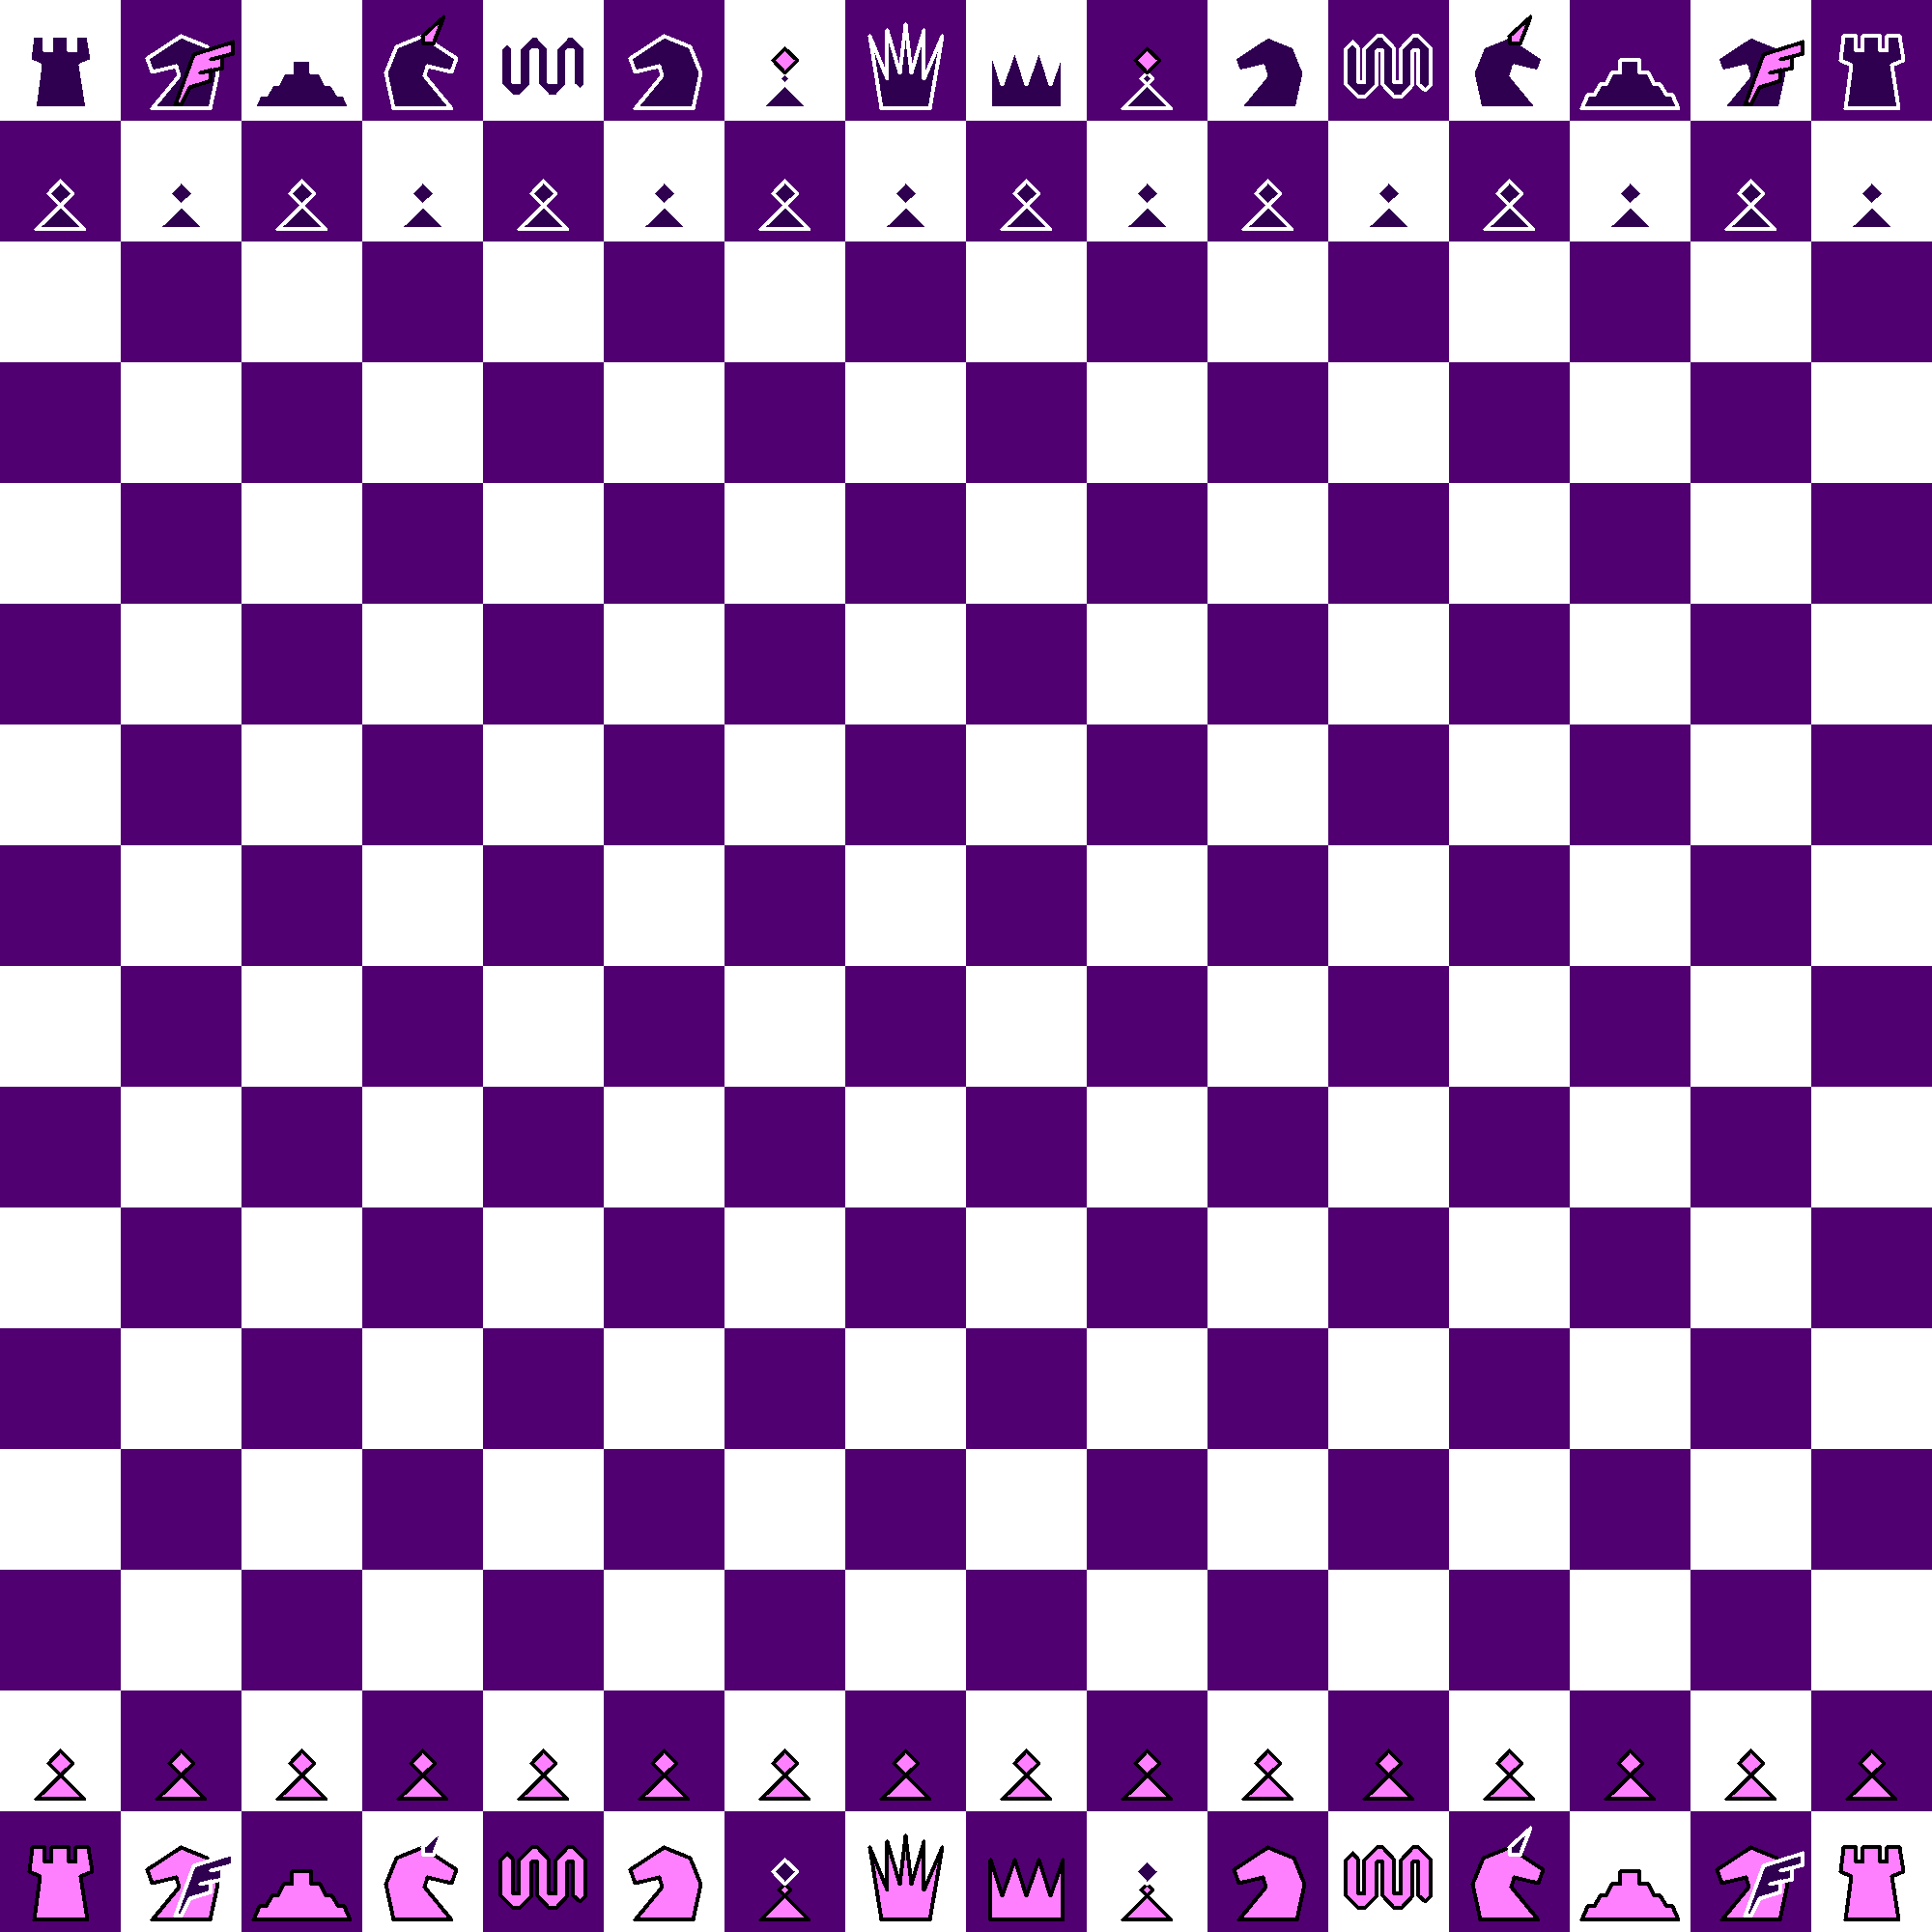
\includegraphics[width=1.0\textwidth, keepaspectratio=true]{boards/10_miranda_s_veil.png}
\caption{Miranda's veil board}
\label{fig:10_miranda_s_veil}
% \centering
\end{figure}

\clearpage % ..........................................................
% ============================================== Miranda's veil chapter
